\chapter{Środowisko}%TODO trochę znikąd. trzebaby opisać najpierw co się dzieje -> tzn coś takiego jak na początku rodziału trzeciego - ze są 3 części i co jak komunikuje się. Niektóre opisy są chyba krótkie... np. o tym co to node.js, że http,, 
Program składa się z trzech głównych elementów:
\begin{itemize}
\item kodu rozszerzającego narzędzie Google Forms (opisanego w 2.1),
\item serwera zaimplementowanego w środowisku Node.js (rozdział 2.2),
\item interfejsu, napisanego przy pomocy HTML i CSS (2.3)
\end{itemize}
\ind Fragmenty kodu korzystają również z bibliotek Pythonowych - skrypt do konwersji sybmoli matematycznych i zdjęć.
\ind Komunikacja pomiędzy elementami pracy wygląda następująco:
\begin{figure}[H]
  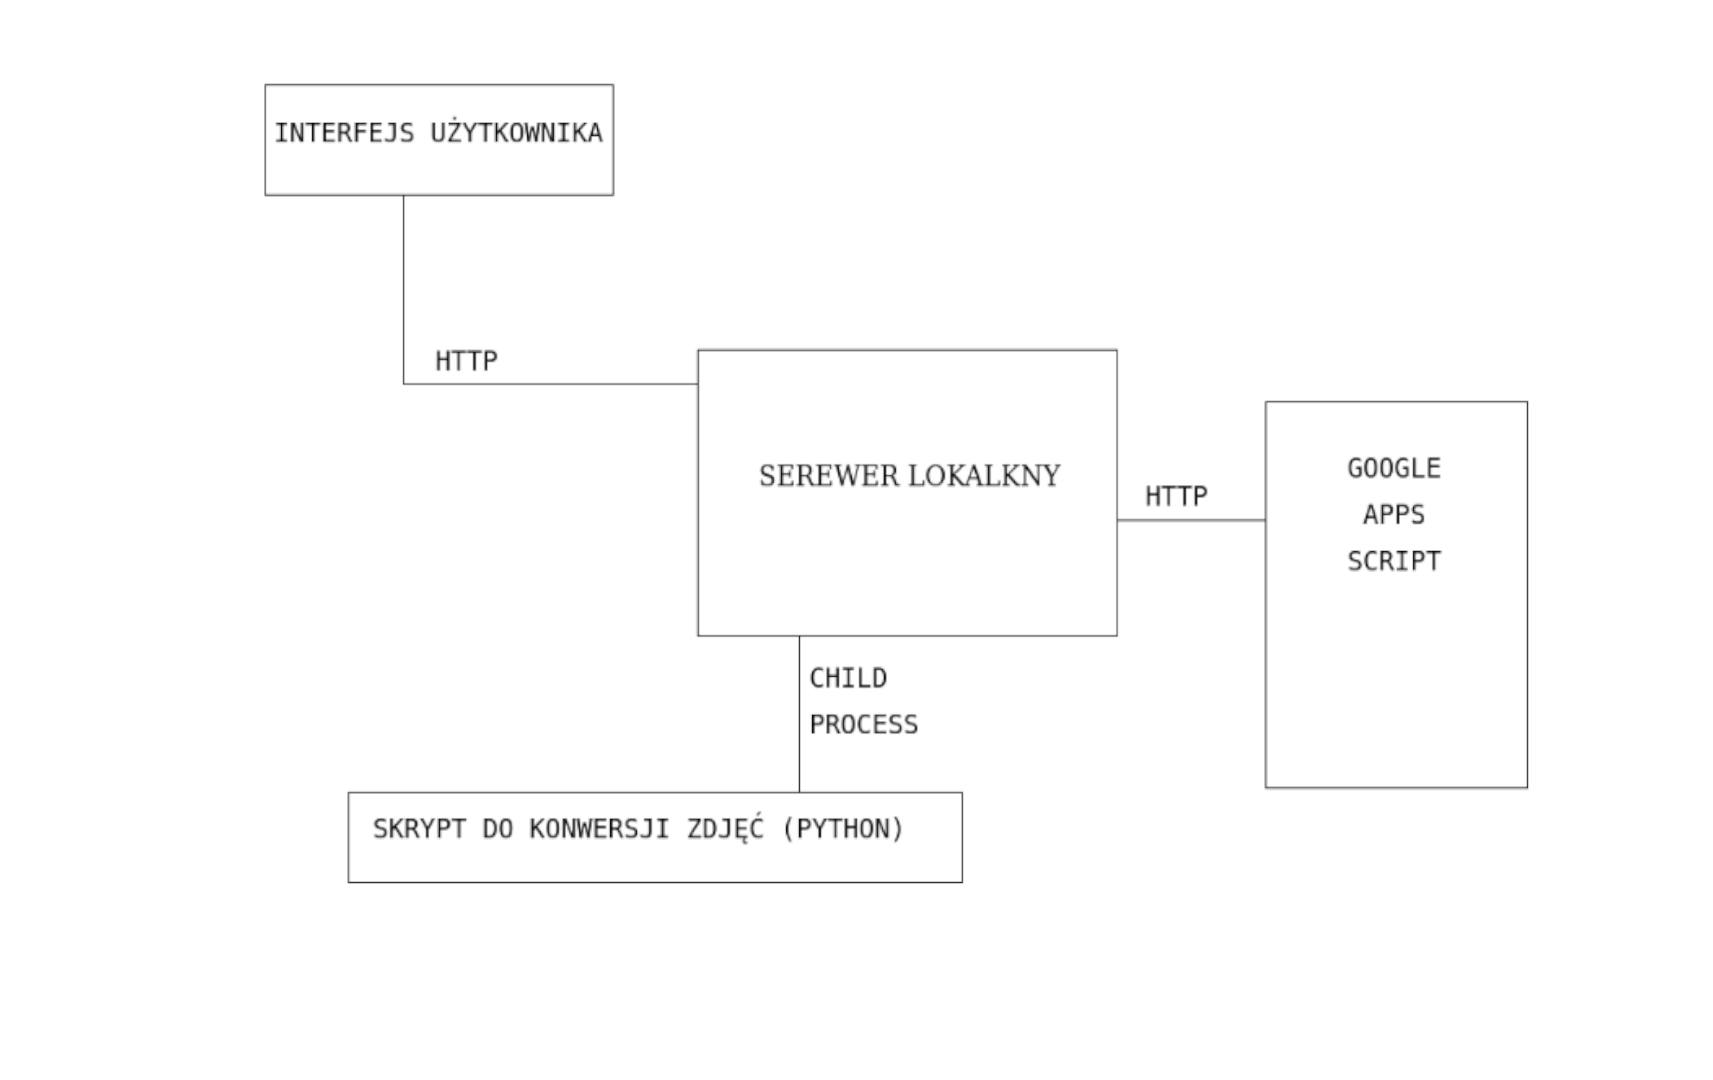
\includegraphics{schemat.png}
  \caption{Schemat połączeń}
  \label{fig:1}
\end{figure}

\section{Google Apps script}
Nabudowywanie na gotowym narzędziu wymaga dostępu do niego. Google udostępnia API operujące na całym szeregu klas i metod oferowanych usług. Kod przypisany jest do danego konta Google, możliwe jest ustawienie parametrów,  takich  jak: kto ma dostęp do nowotworzonej aplikacji internetowej (właściciel, zalogowany użytkownik danej organizacji, dowolny zalogowany użytkownik, każdy) pod czyim kontem jest ona uruchamiana (właściciela/współwłaściciela, czy też zalogowanego użytkownika). 

\paragraph{Framework}
Udostępnione API w pewnym stopniu wymusza na użytkownikach, aby kod wykonywany na infrastrukturze Google'a był napisany w JavaScripcie, we framework'u ,,Google Apps Script''. Program jest wykonywany po stronie serwera. Pozwala on na stosunkowo łatwe manipulowanie działaniem produktów Google takich jak formularze, arkusze, dysk i inne. 
\ind Framework powstał w 2009 roku, w JavaScript 1.6, jest jednak regularnie ulepszany.

\paragraph{Komunikacja}
 Apps Script udostępnia komunikację przez protokół HTTP - jeśli projekt zawiera funkcje doGet(e) / doPost(e) - odpowiednie rządania wykonują kod z ciała tych metod. Zwracane wartości prowadzą do przekierowań zapytań  - automatycznie tworzony jest nowy adres URL. Wysłanie żądania GET pozwala na dotarcie do potrzebnych danych. 
\paragraph{API}
Google Apps Script udostępnia szereg klas i metod związanych z poszczególnymi narzędziami. Szczegółowa dokumentacja narzędzia znajduje się tutaj: \href{https://developers.google.com/apps-script/reference/forms}{Forms Service}.
 Główna klasa - FormApp - jest odpowiedzialna za zarządzanie formularzami - m.in. tworzenie nowych. Każdy typ pytania i element formularza ma odpowiednią klasę (jak np. CheckboxItem czy SectionHeaderItem). Poprzez klasę From  można zmieniać głowne ustawienia formularzy  - jak na przykład dodawanie właściceli, tworzenie pytań, automatyczne ocenianie, manipulowanie tytułem, ustawienie, czy formularz jest ,,aktywny'' (czy przyjmuje odpowiedzi).
 
 
\section{Node.js}
Node.js jest środkowiskiem uruchomieniowym JavaScriptu - stworzonym do tworzenia aplikacji serwerowych. 
Praca wykorzystuje kilka bibliotek, przede wszystkim korzysta jednak z możliwości serwerowych Node.js. 
\paragraph{http}
Interfejs Node.js silnie związany z ,,sercem'' środowiska - udostępnia narzędzia do komunikacji poprzez protokół  HTTP zarówno ze strony serwerowej jak i klienckiej. W pracy w czystej formie wykorzystywany do wysyłania zapytań pomiędzy serwerem lokalnym a serwerem Google'a.
\newline Dokumentacja: \href{https://nodejs.org/api/http.html}{http}
\paragraph{express}
,,Szybki (...), minimalistyczny framework webowy dla Node.js'' - narzędzie pozwala w przystępny sposób postawić serwer (korzysta z biblioteki http). Udostępnia cztery klasy:
\begin{itemize}
\item application - odpowiada aplikacji serwerowej,
\item  request - zarządza odwołaniami do serwera (głównie parametrami),
\item response - odpowiada za odpowiedzi serwera,
\item router - zajmuje się routingiem, może być używane jako oprogramowanie pośredniczące.
\end{itemize}
Trzon kodu narzędzia opiera się właśnie na serwerze express'owym.
\ind Dokumentacja znajduje się tutaj: \href{https://expressjs.com/}{expres.js}
\paragraph{cors}
Node.js'owy moduł pozwalający na odpowiednie ustawienia CORS (Cross-Orgin Request Sharing) w rozwiązaniach typu express. CORS jest metodą rozwiązania problemów z domyślnymi ustawieniami związanymi z bezpieczeństwem. Standardowo dane z jednej strony mogą być pobierane z poziomu drugiej strony gdy obie strony są z tego samego źródła (ten sam schemat Url, host oraz port). CORS pozwala na uniknięcie tej konieczności.
\ind Github modułu: \href{https://github.com/expressjs/cors}{cors}
\paragraph{child\_process}
Moduł Node.js'owy pozwalający na uruchamianie podprocesów. W przypadku omawianego kodu, umożliwa uruchamianie skryptów napisanych  w Pythonie z poziomu kodu Node.js'owego.
\ind Dokumentacja znajduje się tutaj: \href{https://nodejs.org/api/child_process.html}{child\_process}
\paragraph{jsonschema}
\ind Nowy (zaledwie dziesięciomięczny, wciąż w wersji Beta) moduł pozwalający na walidację formatu json zgodnie z podanym schematem.
\ind Oficjalna strona: \href{https://www.npmjs.com/package/jsonschema}{jsonschema}

\section{Python}
Rozwiązania pythonowe zostały wykorzystane w celu konwersji wstawek matematycznych (latex) do zdjęć. Poniżej krótki opis wykorzystanych bibliotek.
\paragraph{tex2pix} Biblioteka pozwalająca na konwertowanie formatu .tex do różnych formatów zdjęciowych. Metoda konwertująca format .tex na format .png zaczyna od konwersji .tex do .pdf, stąd w pracy używana jest konwersja do pdf z tej biblioteki, a dalsze manipulowanie formatem używa innych - subiektywnie prostszych w użytkowaniu - bibliotek. 
\ind Oficjalna strona: \href{https://pypi.org/project/tex2pix/}{tex2pix}.

\paragraph{pdf2image} Biblioteka  umożliwiająca konwersję formatu pdf do formatów zdjęciowych.
\ind Oficjalna strona: \href{https://pypi.org/project/pdf2image/}{pdf2image}.
\paragraph{opencv} Biblioteka pozwalająca na manipulację obrazami. Udostępnia znacznie więcej możliwości niż te użyte w pracy. W szczególności pozwala na przycinanie obrazów względem ich kolorystyki - co pozwala na automatyczne przycięcie strony pdf do rozmiarów napisanego na niej tekstu. Więcej informacji na temat biblioteki: \href{https://pypi.org/project/opencv-python/}{opencv}
\paragraph{base64} Biblioteka pozwala na konwersję obrazu do formatu Base64 - używanego w pracy do przesyłu obrazów pomiędzy serwerami node'owym a google'owym. 

\section{Bootstrap}  
Popularna biblioteka CSS, ułatwiająca budowanie interfejsów graficznych stron internetowych pisanych w HTML. Oficjalna strona \href{https://getbootstrap.com/}{bootstrap}.




